\documentclass[11pt]{article}

\usepackage[english]{babel}                 %% hyphenation rules, spell-checker
\usepackage{amsmath,amssymb}                        %% macros like align* and pmatrix
\usepackage{graphicx,epstopdf}              %% for .eps graphs
\usepackage[official]{eurosym}              %% 1 \euro
\usepackage[a4paper,margin=2cm]{geometry}   %% margins
\usepackage{nameref}
\usepackage{hyperref}                       %% hyperlinks to urls
\usepackage{float}                    

\frenchspacing                              %% no extra space after period
\addtolength{\parskip}{0.5\baselineskip}    %% some white space between paragraphs
\setlength{\parindent}{0pt}                 %% but no indentation
\renewcommand{\baselinestretch}{1.1}        %% line spacing of TeX is small
\DeclareMathOperator{\E}{\mathbb{E}}
\DeclareMathOperator{\Var}{\text{Var}}
\DeclareMathOperator{\Cov}{\text{Cov}}


\title{Non-life --- Assignment NL5}  %% don't forget to change!

\author{
  Niels Keizer\footnote{Student number: 10910492}
  \quad and \quad
  Robert Jan Sopers\footnote{Student number: 0629049}
}

\date{\today}

\begin{document}

\maketitle


\section{The Bornhuetter-Ferguson method}

\subsection*{Q18}

We repeat the code from the assignment, then we extract the \verb|alpha| and \verb|beta| values. Then we check if the sum over the past values obtained from \verb|alpha| and \verb|beta| equals the sum over the fitted values. Finally, we calculate the sum over the future estimated values.

\begin{verbatim}
> Xij <- scan(n=36)
1: 156 37  6  5 3 2 1 0
9: 154 42  8  5 6 3 0
16: 178 63 14  5 3 1
22: 198 56 13 11 2
27: 206 49  9  5
31: 250 85 28
34: 252 44
36: 221
Read 36 items
> TT <- 8; i <- rep(1:TT, TT:1); j <- sequence(TT:1); k <- i+j-1
> fi <- as.factor(i); fj <- as.factor(j); fk <- as.factor(k)
> ee <- c(28950,29754,31141,32443,34700,36268,37032,36637)
> Expo <- rep(ee, TT:1)
> CL <- glm(Xij~fi+fj, quasipoisson)
> EE <- glm(Xij~offset(log(Expo))+fj, quasipoisson)
> 
> cc <- exp(coef(CL))
> alpha <- cc[1] * c(1,cc[2:8]); names(alpha)[1] <- "fi1"
> beta <- c(1,cc[9:15]); names(beta)[1] <- "fj1"
> alpha <- alpha * sum(beta); beta <- beta / sum(beta)
> 
> i_tot <- rep(1:8, each=8)
> j_tot <- rep(1:8,8)
> k_tot <- i_tot+j_tot-1
> future <- k_tot>8
> 
> sum(CL$fitted.values)
[1] 2121
> sum(alpha[i_tot]*beta[j_tot]*!future)
[1] 2121
> sum(alpha[i_tot]*beta[j_tot]*future)
[1] 152.0312
\end{verbatim}

We see that the \verb|alpha| and \verb|beta| give the same past value as the model itself. We also see that we get the results that the assignment says we should get.

The total of the fitted values for past observations equals \verb|sum(Xij)| because of the marginal totals property.

\subsection*{Q19}

We run the code from the assignment and get the following result in \verb|R|.

\begin{verbatim}
> round(tapply(fitted.values(EE)-Xij,j,sum),6)
1 2 3 4 5 6 7 8 
0 0 0 0 0 0 0 0 
\end{verbatim}

The statement in \verb|R| is a sum over the difference between the observed and the fitted values for equal \verb|j|. These are the column sums. Because the \verb|EE| method uses dummy variables for the columns, the marginal totals property holds for the column sums.

\subsection*{Q20}

We execute the following code in \verb|R|, where we replace the dots by \verb|sum(fits) - sum(Xij)|.

\begin{verbatim}
> reserves <- numeric(); lasts <- c(171,181,191,201,211,271,261,251,241,231,221)
> for (last in lasts){
+   Xij[36] <- last
+   cc <- exp(coef(glm(Xij~fi+fj,quasipoisson)))
+   alpha <- c(1,cc[2:TT])*cc[1]; beta <- c(1,cc[(TT+1):(2*TT-1)])
+   fits <- (alpha %o% beta)
+   reserve <- sum(fits) - sum(Xij) ## the sum of the 'future' fitted values
+   reserves <- c(reserves, reserve) 
+ }
> rbind(lasts, reserves=round(reserves))
         [,1] [,2] [,3] [,4] [,5] [,6] [,7] [,8] [,9] [,10] [,11]
lasts     171  181  191  201  211  271  261  251  241   231   221
reserves  132  136  140  144  148  172  168  164  160   156   152
> plot(lasts, reserves); lines(range(lasts),range(reserves))
\end{verbatim}

This results in the following plot:

\begin{figure}[H]\label{fig:q20}
	\centering
	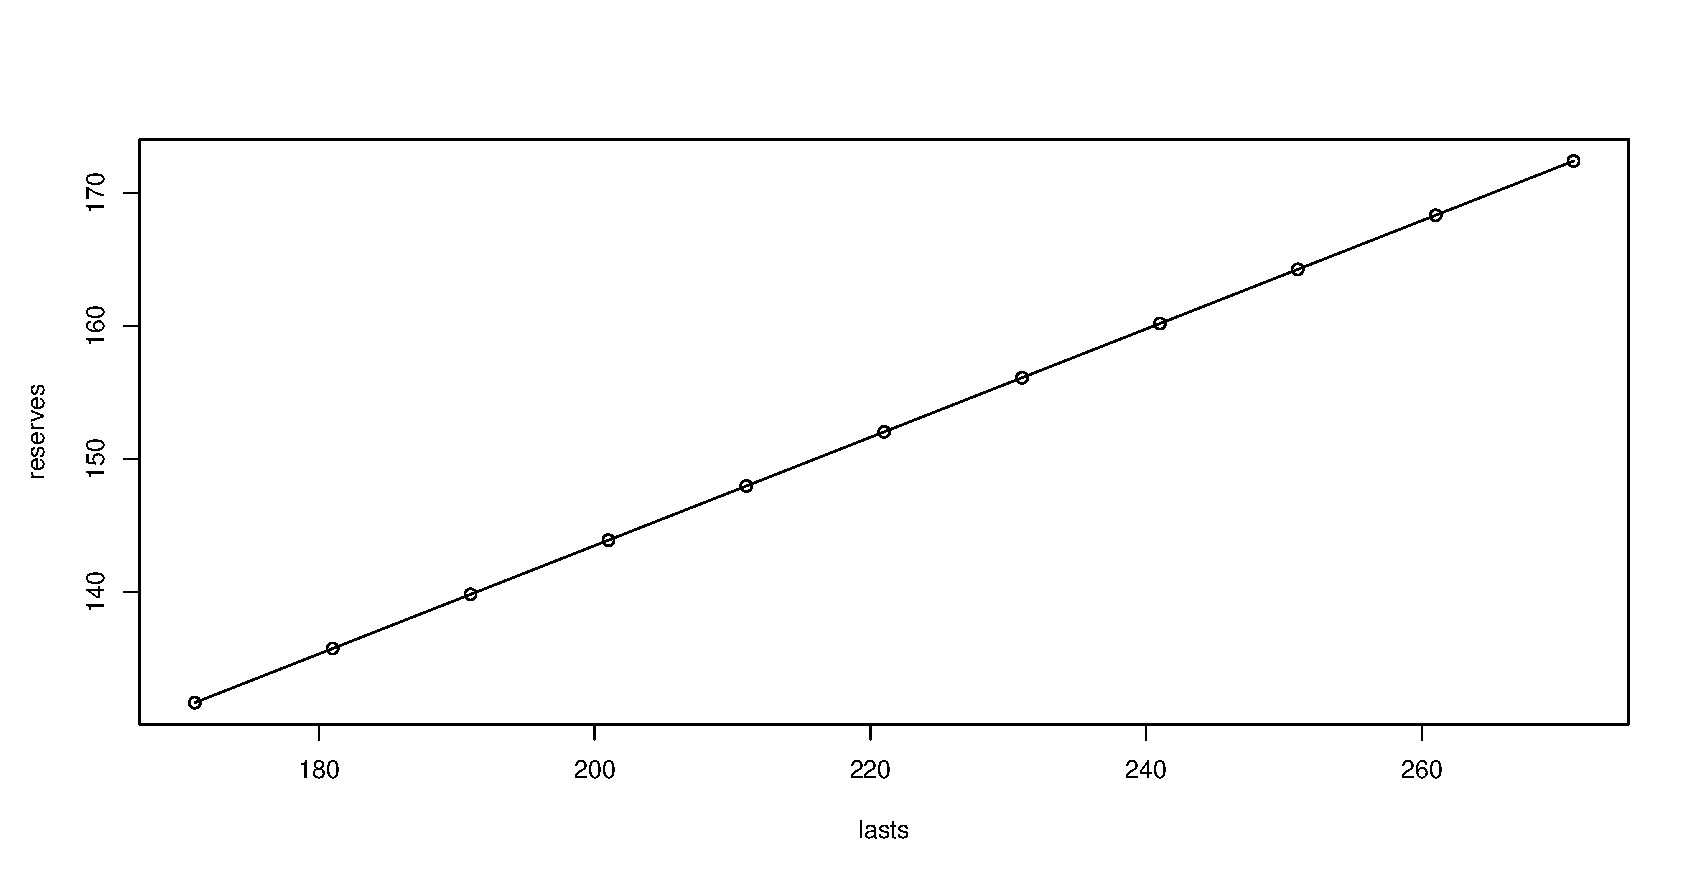
\includegraphics[width=0.8\textwidth]{fig_q20.eps}
	\caption{A plot of the chain ladder reserves against the last claim total.}
\end{figure}

\end{document}
